\documentclass[a4paper,12pt,abstracton]{scrartcl}
\usepackage[ngerman, english]{babel}
\usepackage[utf8]{inputenc}
\usepackage[T1]{fontenc}
\usepackage{graphicx}
\usepackage{lipsum}
\usepackage{blindtext}

\title{Bachelorarbeit}
\author{Sophia Milanov}
\date{\today}

\begin{document}

\begin{titlepage}
\begin{center}
 
\Large\textbf{Department of Physics and Astronomy\\
University of Heidelberg}

\vspace{16cm}

\normalsize
Bachelor Thesis in Physics\\
submitted by \\
\vspace{0.5cm}
\Large\textbf{Sophia Milanov}\\
\normalsize
\vspace{0.5cm}
born in Düsseldorf (Germany)\\
\vspace{0.5cm}
\Large\textbf{2016}
\normalsize

\newpage




\Large\textbf{Title}

\vspace{18cm}

\normalsize
This Bachelor Thesis has been carried out by Sophia Milanov at the\\
Max Planck Institute for Astronomy in Heidelberg\\
under the supervision of\\
Dr. Glenn van de Ven

\vfill
\end{center}

\end{titlepage}


\begin{abstract}
\blindtext 
\end{abstract}

\newpage

\tableofcontents

\newpage
\section{Introduction}
\subsection{motivation}
\subsection{What is a globular cluster in the Milky Way?}
150 of them \\
kugelförmige anordnung von Sternen 10**6 bis 10**8\\
große frage: IMBHs ja/nein\\
stellar population with plot of cmd (characteristics of each stage) without isochrones explaining the different evolution stages and binaries included and refer to 3.1.

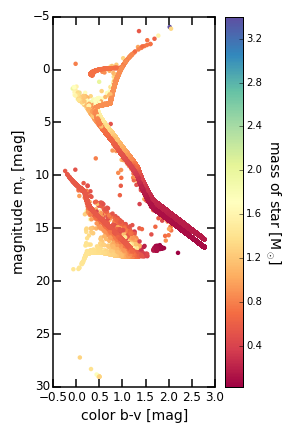
\includegraphics[width=\textwidth]{Plots/color_magnitude_diagram}
\subsection{Actions\&orbits}
integral of motion\\
klarste beschreibung des orbits\\
actions zeitlich konstant\\
schon lange sind actions bekannt\\
auch vom sonnensystem\\
für andere extrem schwierig zu berechnen\\
mit supercomputern endlich möglich


\newpage
\section{Method \& Theory}
%\subsection{stellar population in GC}
\subsection{observed kinematics in GCs}
\subsection{Orbits}
Poisson's equation
density \& potent
\subsection{actions}
\newpage
\section{Analysis}

\subsection{Description of the simulation}
where simulation comes from and what it is \& description of output\\
x-y-z plot how it looks like\\
test of sphericity \& center\\
cmd with isochrones explaining them and showing that they fit with the simulation\\

\subsection{Investigation in phase space}
Paolo class

\subsubsection{Velocity dispersion}
aussage\\
plots\\
erklärung physikalisch
\subsubsection{anisotropy}
\subsubsection{Density profile}
plots\\
bestätigung kugelförmig\\
potential daraus
\subsubsection{Potential}

\subsection{Investigations of orbits in action space}
wilma class 
\subsubsection{Orbits}
\subsubsection{Actions}
\subsubsection{Integral of motions along orbits}
\newpage
\section{Results \& Discussion}
only triangle plots

\subsection{Actions from different globular clusters}
\subsection{Discussion \& future perspectives}
do the same distinguishing the mass of the stars\\
redo the work with only observational light data
\newpage
\section{Conclusion}
\end{document}